%------------------------------------------------------------------------------
% Author(s):
% Varaun Ramgoolie
% Copyright:
%  Copyright (C) 2020 Brad Bachu, Arjun Mohammed, Nicholas Sammy, Kerry Singh
%
%  This file is part of Applied-Mathematics-Unit2 and is distributed under the
%  terms of the MIT License. See the LICENSE file for details.
%
%  Description:
%     Year: 2008 May
%     Module: 1
%     Question: 1 
%------------------------------------------------------------------------------
\usetikzlibrary{patterns}

\begin{subquestions}
	
%------------------------------------------------------------------------------
% 1 a--------------------------------------------------------------------------
%------------------------------------------------------------------------------

\subquestion

Let $x$ be the number of newspaper advertisements and let $y$ be the number of television advertisements.	

The objective function that we want to maximize is,

\begin{equation}
	C =2x+5y \,.
\end{equation} 

The constraints of this linear programming model are as follows,

\begin{align}
	1500x + 5000y & \leq 5000 \,, \nn \\
	1500x & \leq 30000 \,, \nn \\
	5000y & \geq 25000 \,, \nn \\
	x & \leq 2y \,.
\end{align}

%------------------------------------------------------------------------------
% 1 b--------------------------------------------------------------------------
%------------------------------------------------------------------------------

\subquestion

\begin{subsubquestions}

%-----------------------------------------------------------------------------
	
\subsubquestion

The feasible region is shaded in the graph below.

\begin{center}
	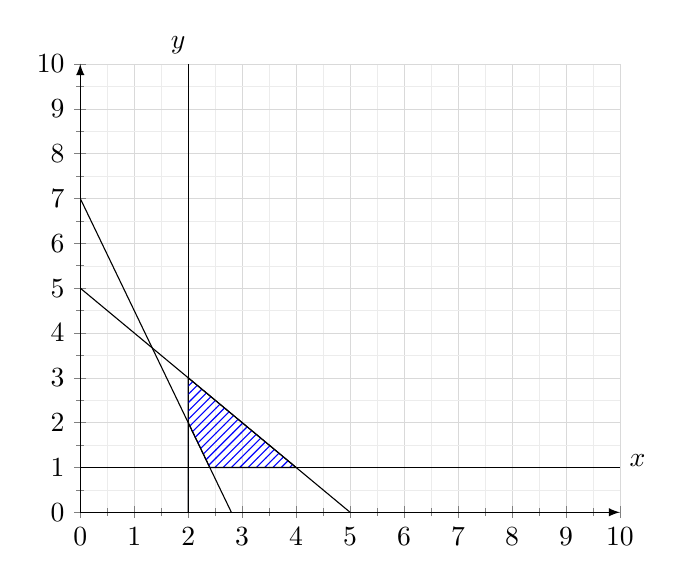
\begin{tikzpicture}
		\begin{axis}
			[
			xmin=-0,xmax=10,
			ymin=0,ymax=10,
			grid=both,
			grid style={line width=.1pt, draw=darkgray!10},
			major grid style={line width=.2pt,draw=darkgray!20},
			axis lines=left,
			minor tick num=1,
			enlargelimits={abs=0},
			axis line style={-latex},
			samples=100,
			domain = -20:20,
			ytick={0,1,...,10},
			xtick={0,1,...,10},
			xlabel={$x$},
			ylabel={$y$},
			x label style={at={(axis description cs:1,0.15)},anchor=north west},
			y label style={at={(axis description cs:0.15,1)},anchor=south west, rotate=-90}
			]
			
			\addplot [mark=dot] coordinates{(5, 0)  (0,5)} {};
			
			\addplot [mark=dot] coordinates {(2.8,0) (0, 7)} {};
			
			\addplot [mark=dot] coordinates {(2,0) (2, 10)} {};
			
			\addplot [mark=dot] coordinates {(0, 1) (10, 1)} {};
			
			\addplot [pattern=north east lines,pattern color=blue] coordinates {(2,2) (2, 3) (4, 1) (2.4,1) (2,2)} \closedcycle;	
				
		\end{axis}	
	\end{tikzpicture}
\end{center}

%-----------------------------------------------------------------------------------------

\subsubquestion

Using \rdef{mod1:defn:TourOfVertices},

\begin{align}
	\text{Using (2,2)} \,, \nn \\
	P & = 2x + 7y \,, \nn \\
	& = (2 \times 2) + (7 \times 2) \,, \nn \\
	& = 18 \,. \\
	\text{Using (2,3)} \,, \nn \\
	P & = 2x + 7y \,, \nn \\
	& = (2 \times 2) + (7 \times 3) \,, \nn \\
	& = 25 \,. \\  \label{2012:q1:eqn:Profit}	  
	\text{Using (4,1)} \,, \nn \\
	P & = 2x + 7y \,, \nn \\
	& = (2 \times 4) + (7 \times 1) \,, \nn \\
	& = 15 \,.  \\
	\text{Using (2.4, 1)} \,, \nn \\
	P & = 2x + 7y \,, \nn \\
	& = (2 \times 2.4) + (7 \times 1) \,, \nn \\
	& = 11.8 \,. 
\end{align}

Thus, the maximum value of $P$ is $25$.

\end{subsubquestions}

\end{subquestions}

